%%%%%%%%%%%%%%%%%%%%%%%%%%%%%%%%%%%%%%%%%
% Journal Article
% LaTeX Template
% Version 1.4 (15/5/16)
%
% This template has been downloaded from:
% http://www.LaTeXTemplates.com
%
% Original author:
% Frits Wenneker (http://www.howtotex.com) with extensive modifications by
% Vel (vel@LaTeXTemplates.com)
%
% License:
% CC BY-NC-SA 3.0 (http://creativecommons.org/licenses/by-nc-sa/3.0/)
%
%%%%%%%%%%%%%%%%%%%%%%%%%%%%%%%%%%%%%%%%%

%----------------------------------------------------------------------------------------
%	PACKAGES AND OTHER DOCUMENT CONFIGURATIONS
%----------------------------------------------------------------------------------------

\documentclass[twoside,twocolumn]{article}

\usepackage[sc]{mathpazo} % Use the Palatino font
\usepackage[T1]{fontenc} % Use 8-bit encoding that has 256 glyphs
\linespread{1.05} % Line spacing - Palatino needs more space between lines
\usepackage{microtype} % Slightly tweak font spacing for aesthetics

\usepackage[utf8]{inputenc}
\usepackage[spanish]{babel} % Language hyphenation and typographical rules

\usepackage[hmarginratio=1:1,top=32mm,columnsep=20pt]{geometry} % Document margins
\usepackage[hang, small,labelfont=bf,up,textfont=it,up]{caption} % Custom captions under/above floats in tables or figures
\usepackage{booktabs} % Horizontal rules in tables

\usepackage{lettrine} % The lettrine is the first enlarged letter at the beginning of the text

\usepackage{enumitem} % Customized lists
\setlist[itemize]{noitemsep} % Make itemize lists more compact

\usepackage{abstract} % Allows abstract customization
\renewcommand{\abstractnamefont}{\normalfont\bfseries} % Set the "Abstract" text to bold
\renewcommand{\abstracttextfont}{\normalfont\small\itshape} % Set the abstract itself to small italic text

\usepackage{titlesec} % Allows customization of titles
\renewcommand\thesection{\Roman{section}} % Roman numerals for the sections
\renewcommand\thesubsection{\roman{subsection}} % roman numerals for subsections
\titleformat{\section}[block]{\large\scshape\centering}{\thesection.}{1em}{} % Change the look of the section titles
\titleformat{\subsection}[block]{\large}{\thesubsection.}{1em}{} % Change the look of the section titles

\usepackage{fancyhdr} % Headers and footers
\pagestyle{fancy} % All pages have headers and footers
\fancyhead{} % Blank out the default header
\fancyfoot{} % Blank out the default footer
\fancyhead[C]{Teoría de las comunicaciones $\bullet$ Mayo 2017} % Custom header text
\fancyfoot[RO,LE]{\thepage} % Custom footer text

\usepackage{titling} % Customizing the title section

\usepackage{hyperref} % For hyperlinks in the PDF

%----------------------------------------------------------------------------------------
%	TITLE SECTION
%----------------------------------------------------------------------------------------

\setlength{\droptitle}{-4\baselineskip} % Move the title up

\pretitle{\begin{center}\Huge\bfseries} % Article title formatting
\posttitle{\end{center}} % Article title closing formatting
\title{TP1: Wiretapping} % Article title
\author{
\textsc{Fabio Seminara} \\
\textsc{Matías Millassón} \\
\textsc{Lautaro Leonel Alvarez} \\
\\
\normalsize FCEN - Universidad de Buenos Aires
}
\date{\today} % Leave empty to omit a date
\renewcommand{\maketitlehookd}{
\begin{abstract}
\noindent Una descripción corta del tp, de qué vamos a explicar y sobre qué experimentamos.
\end{abstract}
}

%----------------------------------------------------------------------------------------

\begin{document}

% Print the title
\maketitle

%----------------------------------------------------------------------------------------
%	ARTICLE CONTENTS
%----------------------------------------------------------------------------------------

%\section{Capturando tráfico}
%Acá habría que explicar la implementación y por qué capturamos esos paquetes, si cambiamos, probamos, etc.


%\section{Analizando los paquetes capturados}
\section{Introducci\'on}
\section{Introducción}

\par En el siguiente trabajo práctico vamos a análizar 3 redes locales con el fin de caracterizarlas en base a los nodos que participan enviando o recibiendo paquetes, la cantidad de paquetes y el rol que cumplen (o creemos que cumplen) dentro de la red. Para esto, utilizaremos un \textit{sniffer} que escucha la red y almacena los datos recolectados.
\par Antes que nada, daremos unos conceptos importantes sobre el tema para poder explicar mejor el funcionamiento y alcance de esta herramienta.

\subsection{ARP: Adress Resolution Protocol}

\par Es el protocolo encargado de mapear direcciones del nivel 3 al nivel 2. Los paquetes ARP poseen varios campos de información pero en este trabajo solo nos van a interesar la dirección MAC e IP destino y fuente y el tipo de mensaje, es decir si es who-has o is-at.
\par Cuando un equipo quiere comunicarse con otro envía un paquete ARP de tipo who-has (broadcast) y el equipo buscado responde con un paquete ARP de tipo is-at (unicast). Estos envíos sirven para que cada equipo arme su propia tabla ARP en la cual asocia direcciones IP con direcciones MAC.

\subsection{Modo promiscuo}

\par Se trata de una configuración de la placa de red, en la cual transmite a sus niveles superiores todos los paquetes que escucha, y no solo los que van dirigidos a nuestra pc (como pasa normalmente). La herramienta sniffer utiliza precisamente este modo para tomar todos los paquetes que logre leer.

\subsection{Teoría de la información}

\par Vamos a usar la teoría estadística de la información (o teoría de Shannon). Sin entrar tan en detalle, nos interesarán las siguientes definiciones:

\begin{itemize}
  \item \textbf{Información de un suceso:} Dado un suceso $i$ de una fuente cuya probabilidad es estrictamente mayor que cero se define su información como $c_i $= $-log(p_i)$ con $p_i$ la probabilidad de que ocurra el suceso $i$. Se puede observar que cuanto menos probable sea un suceso más información provee y cuanto más probable sea menos información aporta.
  \item \textbf{Entropía de una fuente:} Dada una fuente $S$ se define la entropía como $H(S)$ = $\sum_{i=1}^{\#(S)} p_i*c_i$ con $c_i$ la información del suceso $i$ y $p_i$ su probabilidad. Esta m\'etrica es un promedio ponderado de la información que brinda cada suceso.
\end{itemize}

\subsection{Herramienta sniffer}
\par Ahora sí, podemos pasar a definir la herramienta que desarrollamos y una breve introducción a su funcionamiento. La herramienta utiliza una librería llamada scapy\footnote{SCAPY: https://github.com/secdev/scapy/}, que es la encargada de pasar al sistema a modo promiscuo y obtener todos los paquetes que pueda identificar. De esta manera, luego de obtener estos paquetes, se calculan la información y entropía de distintas fuentes de información (que luego mencionaremos) y al mismo tiempo se almacena la información que consideramos relevante en un archivo de salida (para poder ser utilizado luego).

\subsection{Fuentes de información analizadas}
\par Para analizar los datos de paquetes obtenidos por la herramienta definimos dos fuentes de información:
\begin{itemize}
  \item \textbf{S:} El conjunto de símbolos definidos es $\{S_{broadcast},S_{Unicast}\}$. El símbolo $S_{broadcast}$ corresponde a los paquetes capturados cuya dirección de destino es ff:ff:ff:ff:ff:ff, mientras que el resto de los paquetes van a ser considerados $S_{unicast}$.
  \item \textbf{S1:} El conjunto de símbolos definidos son todas las direcciones IPv4 que tuvieron todos los dispositivos mientras estaban conectados a la red. En esta fuente sólo consideramos los paquetes de tipo \textbf{who-has}.
\end{itemize}


\subsection{Experimento 1}
\section{Primera captura: Laboratorio de Pabellón 1}

\par Para una primera experimentación, decidimos correr la herramienta sniffer en la red interna del pabellón 1 de Ciudad Universitaria. Nos conectamos por Wifi a la red y tomamos muestras durante 17 minutos. Utilizamos la fuente de información S1 para diferenciar cada host como un símbolo. Luego, calculamos la información de cada host y con esto, la entropía de la fuente (red).

\subsection{Resultados y análisis}

\par En el gráfico \ref{fig:exp1_labo_infovsentro} se pueden ver los 25 hosts con menor información. La linea punteada roja representa la entropía de la fuente y, como se observa rápidamente, hay un solo host que se encuentra del lado izquierdo (\textbf{10.210.210.199}). Esto significa que es un símbolo con muy poca información y por ende, mucha probabilidad. Para nosotros, esto significa que es un host que participa mucho de la red, preguntando constantemente qué dirección MAC corresponde a una dirección IP. Tomamos entonces a este host como un nodo distinguido de la red.

\begin{figure}[h]
  \begin{subfigure}{.5\textwidth}
    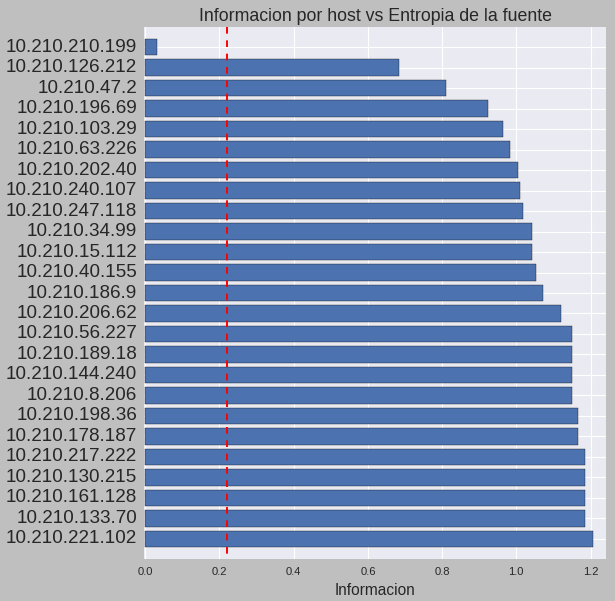
\includegraphics[width=\textwidth]{imagenes/laboratorio/informaciones_vs_entropia.png}
  \end{subfigure}
  \label{fig:exp1_labo_infovsentro}
  \caption{Información de cada símbolo (host) de la red comparada con el valor de la entropía de la fuente de información (red local). Se limita el gráfico a los 25 símbolos con menor valor de información.}
\end{figure}

\begin{figure*}[ht]
  \hspace*{-0.5cm}
  \begin{subfigure}{1.1\textwidth}
    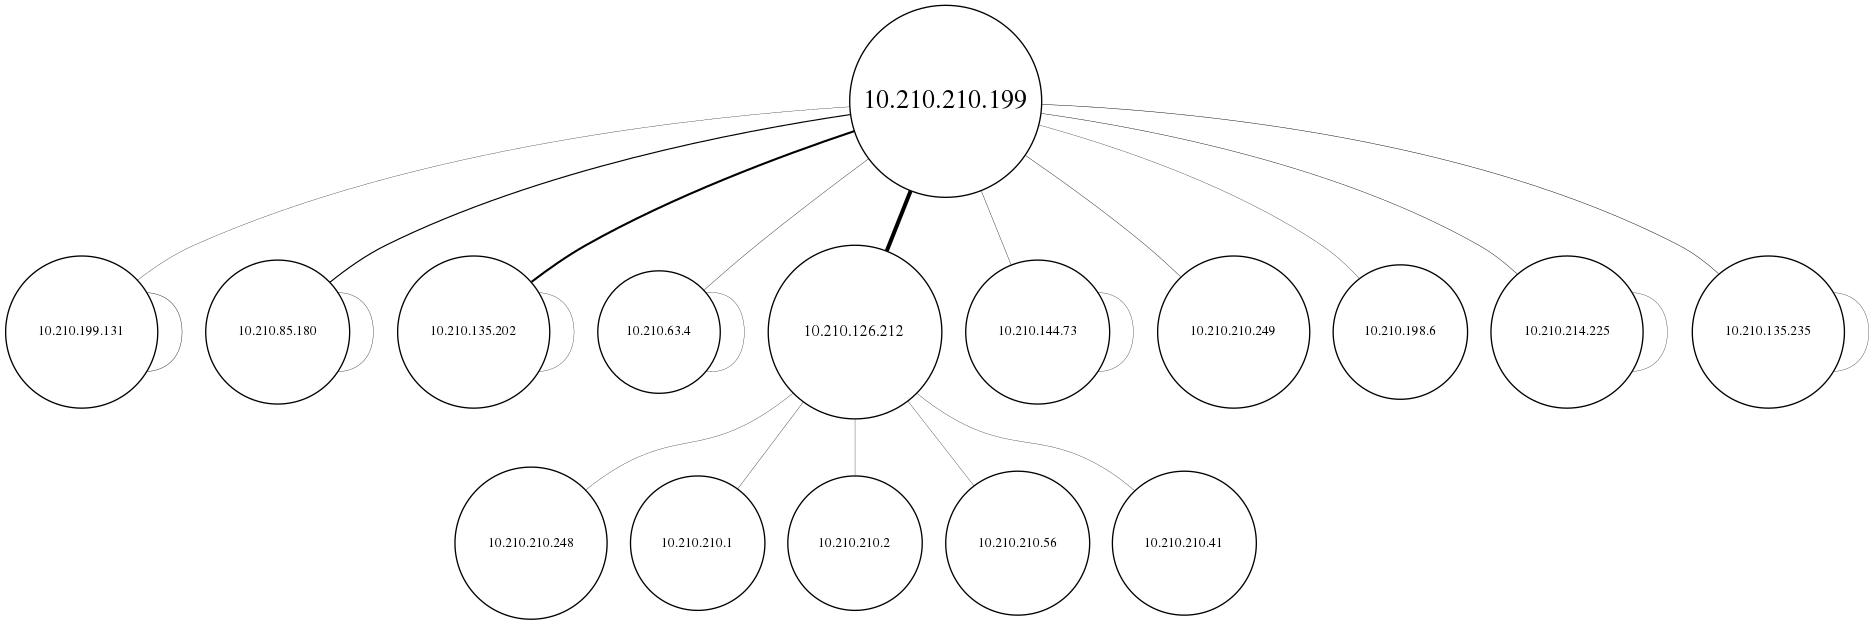
\includegraphics[width=\textwidth]{imagenes/laboratorio/grafo_10.png}
  \end{subfigure}
	\label{fig:exp1_labo_grafo}
	\caption{Grafo con los nodos mas interesantes de la red de la primer captura. El diámetro del nodo implica mayor participación.}
\end{figure*}

\par La distinción del host con IP \textbf{10.210.210.199} la podemos corroborar en el gráfico de la figura \ref{fig:exp1_labo_grafo}. Este grafo representa a la red relacionando nodos con hosts y aristas con mensajes. El diámetro de los nodos está dado por el nivel de participación que tiene en la captura tomada. Asimismo, se obviaron muchos nodos con comportamiento similar que no sumaban valor al grafo, asegurando que los mas \textit{participativos} se mantengan. Este valor de \textit{participación} fue calculado teniendo en cuenta los siguientes parámetros:

\begin{enumerate}
	\item Cantidad de mensajes ARP enviados (solo tomando los del tipo who-has).
	\item Cantidad de mensajes ARP que consultaban por su ip (solo tomando los del tipo who-has).
	\item Cantidad de hosts \textit{distintos} por los cuales preguntó su dirección MAC.
	\item Cantidad de hosts \textit{distintos} que preguntaron por su dirección MAC.
\end{enumerate}

\par A estos 4 parámetros se les asigna un peso, que depende de lo que queramos observar. En este caso en particular, los parámetros 1 y 2 tienen peso 0 porque queríamos enfocarnos en los 3 y 4, que en cierta forma implican a los 1 y 2 (si la cantidad de \textit{distintos} es grande, esto implica que la cantidad sin tener en cuenta distinción de hosts también es grande). Al parámetro 3 le asignamos peso 2, mientras que al 4 le asignamos peso 10. De esta manera, podemos destacar fuertemente los hosts por los cuales muchos otros consultaron por él, pero también teniendo en cuenta (con menor importancia) los hosts que consultaron por muchas direcciones. Lo que logramos con estos valores, es lo que observamos en el grafo de la figura \ref{fig:exp1_labo_grafo}.
\par Las aristas por su parte, representan la consulta de un host por la dirección MAC de otro (sin diferenciar la dirección de los mensajes). Y el peso de cada arista (relacionado con el grosor) está dado por la cantidad de mensajes que relacionan a los hosts.
\par Observando este grafo, notamos que el host con IP \textbf{10.210.126.212} tiene un comportamiento particular. Para analizar mejor la situación vamos a referirnos al host con IP \textbf{10.210.210.199} como \textbf{Nodo A} y al host con IP \textbf{10.210.126.212} como \textbf{Nodo B}. A continuación vamos a mencionar información que extrajimos de la muestra y luego pasaremos a analizar el por qué de estos valores y tratar de caracterizar los nodos según su comportamiento:

\begin{itemize}
  \item Solo el nodo A preguntó por la dirección del nodo B, y lo hizo 121 veces.
  \item El nodo B nunca preguntó por la dirección del nodo A, mientras que otros 268 hosts si lo hicieron.
  \item El nodo A realizó 5796 preguntas, por 298 direcciones distintas (entre ellas la ip del nodo B).
  \item El nodo B realizó 151 preguntas, por 101 direcciones distintas.
\end{itemize}

\begin{figure}[h]
  \begin{subfigure}{.5\textwidth}
    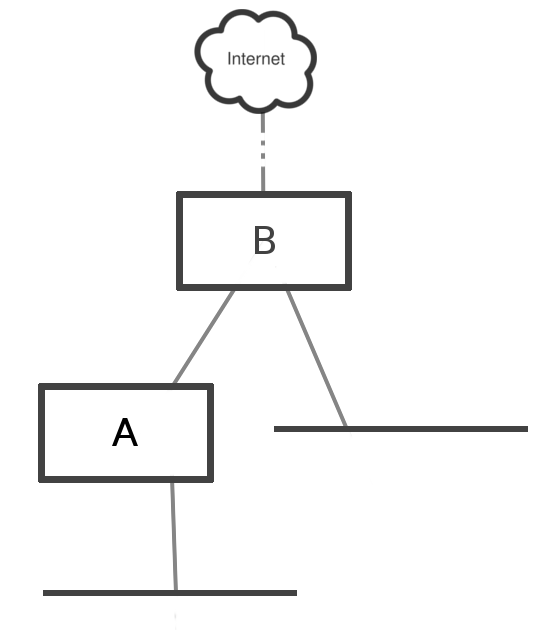
\includegraphics[width=\textwidth]{imagenes/laboratorio/red.png}
  \end{subfigure}
  \label{fig:exp1_labo_red}
  \caption{Diagrama de cómo creemos que está organizada la red de la primera captura.}
\end{figure}

\subsection{Conclusiones}

\par Por esta información, creemos que el nodo A es un access point de la red Wifi, ya que tiene interacción con muchos hosts (entre 268 y 297) y la gran mayoría de ellos solo preguntan por él. Y en el caso del nodo B, creemos que es algún router por el cual debe acceder el nodo A para poder salir a internet. Al mismo tiempo, el nodo B tiene interacción con bastantes hosts (151). También vemos que no tienen interacciones en común (quienes preguntan por A no preguntan por B, y la inversa). Por esto, creemos que el nodo B debe ser el gateway de otra red local. En la figura \ref{fig:exp1_labo_red} planteamos la idea de lo que creemos que puede ser la red, dejando varios interrogantes, pero dando una idea general de su organización.

\subsection{Experimento 2}
\begin{figure*}[ht]
  \hspace*{-0.5cm}
  \begin{subfigure}{1.1\textwidth}
    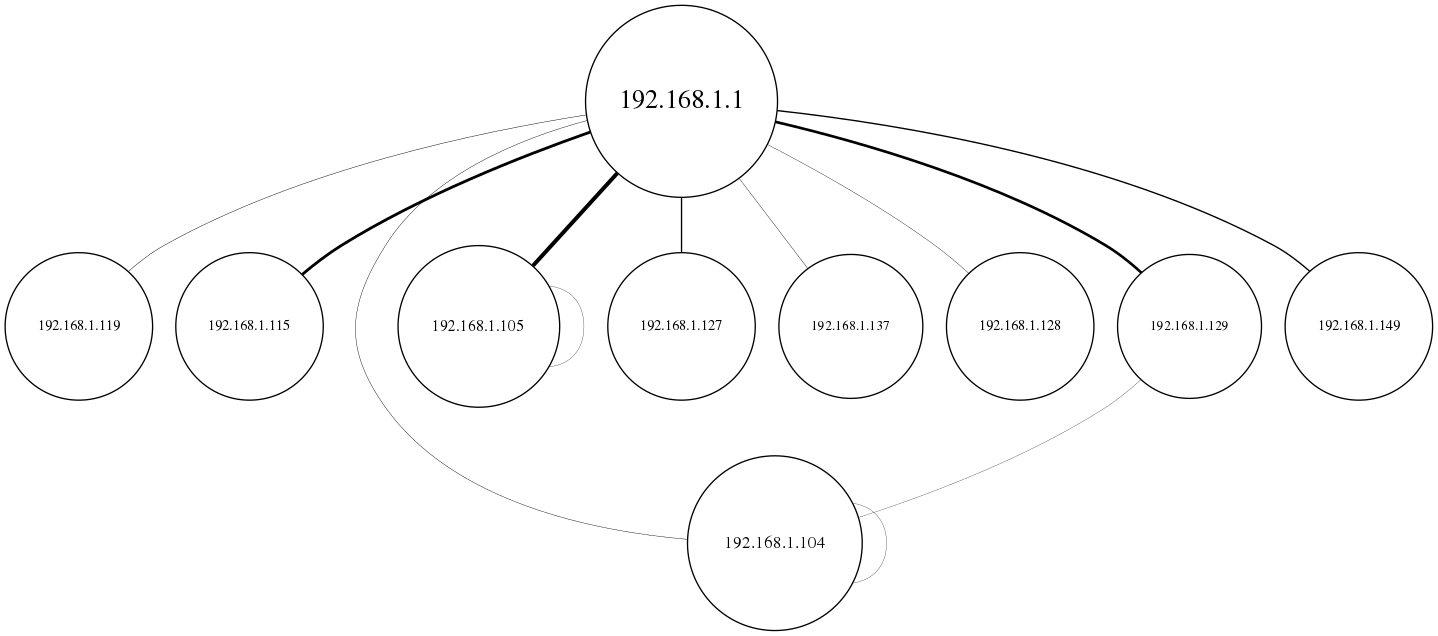
\includegraphics[width=\textwidth]{imagenes/hogarenia/grafo.png}
  \end{subfigure}
	\label{fig:exp2_hogar_grafo}
	\caption{Grafo con los nodos de la red de la segunda captura. El diámetro del nodo implica mayor participación en el envío de paquetes.}
\end{figure*}

\section{Segunda Captura: Red local chica}

\par Para una segunda experimentación, tomamos una captura de una red casera por medio de la herramienta sniffer antes mencionada. Se capturaron mensajes durante 2 horas y al ser una red pequeña, a diferencia del primer experimento, vamos a analizar tanto la fuente de información S como la S1.

\subsection{Resultados y análisis}

\par En el gráfico de la figura \ref{fig:exp2_hogar_hosts_infovsentro} podemos observar la información de cada símbolo (host) en la fuente S1. Se puede ver claramente que hay un solo host que se encuentra a la izquierda de la linea punteada roja, que representa la entropía de la red. Este host con IP \textbf{198.168.1.1} va a ser para nosotros un nodo distinguido, ya que participa fuértemente en los mensajes ARP que se envían en la red y por esto, tiene un valor de información pequeño.

\begin{figure}[h]
  \begin{subfigure}{.5\textwidth}
    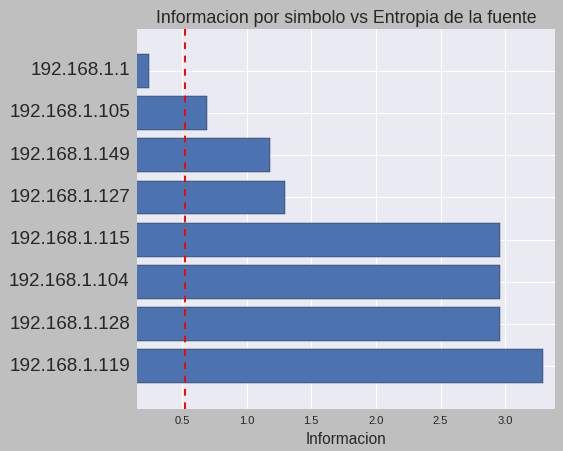
\includegraphics[width=\textwidth]{imagenes/hogarenia/hosts_informaciones_vs_entropia.png}
  \end{subfigure}
  \label{fig:exp2_hogar_hosts_infovsentro}
  \caption{Información de cada símbolo (host) comparada con el valor de la entropía de la fuente de información (red local).}
\end{figure}

\par Con respecto a la fuente de información S, tenemos el gráfico de la figura \ref{fig:exp2_hogar_brvsun_infovsentro}. En este gráfico observamos la información del símbolo \textit{Unicast} y el símbolo \textit{Broadcast}. Podemos notar que el símbolo \textit{Unicast} supera ampliamente al símbolo \textit{Broadcast}. Esto significa que se identificaron una cantidad elevada de mensajes del tipo \textit{Broadcast} en la red.

\begin{figure}[h]
  \begin{subfigure}{.5\textwidth}
    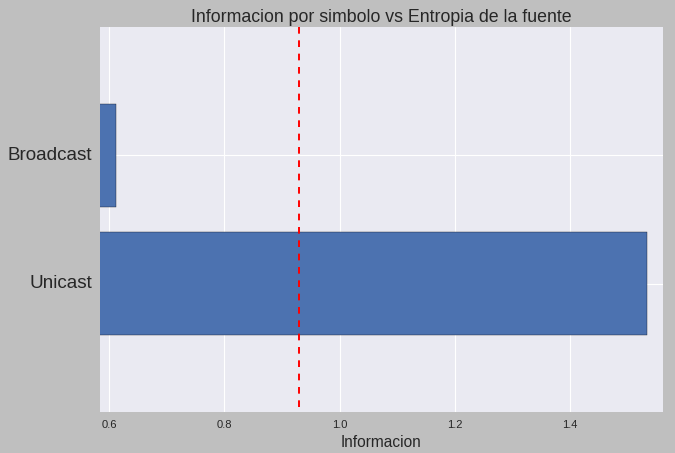
\includegraphics[width=\textwidth]{imagenes/hogarenia/brvsun_informaciones_vs_entropia.png}
  \end{subfigure}
  \label{fig:exp2_hogar_brvsun_infovsentro}
  \caption{Información de cada símbolo (Broadcas / Unicast) comparada con el valor de la entropía de la fuente de información (red local).}
\end{figure}

\par El grafo de la figura \ref{fig:exp2_hogar_grafo} es una representación de la red de acuerdo a los hosts identificados y las relaciones entre ellos (dadas por mensajes ARP que consultan direcciones entre ellos). El tamaño de los nodos, al igual que en la primer captura, está relacionado con la \textit{participación} que tienen en la red. Aquí también podemos notar que el host con IP \textbf{192.168.1.1} es el que mas participa de los mensajes ARP. También podemos notar que todos los otros hosts se encuentran unidos a él (preguntaron por su dirección o la inversa). De el mismo grafo, podemos ver también que los hosts \textbf{192.168.1.104} y \textbf{192.168.1.129} se encuentran conectados, mientras que todo el resto solo se conectan con el host \textbf{192.168.1.1}. Luego de corroborar los datos, notamos que hay un mensaje ARP que emitió el host \textbf{192.168.1.104} preguntando por la dirección del host \textbf{192.168.1.129}.

\subsection{Conclusiones}

\par Como observamos en el grafo y corroboramos con la información del símbolo en la fuente de información S, el host \textbf{192.168.1.1} se encuentra conectado con todos los otros hosts, por lo que creemos que es un router o access point con el cual el resto de los hosts se comunican. El resto de los hosts, nos resultan similares y no creemos que sean hosts destacados o distinguidos.

\subsection{Experimento 3}
\section{Tercer captura: Red local muy chica}

\par Se realizó una tercer captura en una red local que poseía solamente tres hosts. La captura duró aproximadamente veinte minutos. En este caso vamos a analizar ambas fuentes de información.
\par En este experimento se tuvo una red con tres hosts, uno es el router (\textbf{192.168.1.1}), otro es dónde se estaba ejecutando la herramienta de monitoreo (\textbf{192.168.1.124}) mientras que en el equipo restante se estuvo realizando una descarga mediante un cliente torrent durante casi todo el tiempo (\textbf{192.168.1.129}).

\subsection{Resultados y análisis}

\par En el gráfico de barras en el que se compara la información de cada símbolo la fuente S con la entropía de la misma (figura 8) se puede ver que, al igual que en los demás experimentos hubo muchísimos más paquetes \textit{Broadcast} que \textit{Unicast}. Aún así el valor de la entropía está bastante cerca de ser el máximo, el cual es 0.5 ya que son dos símbolos.

\begin{figure}[h]
  \begin{subfigure}{.5\textwidth}
    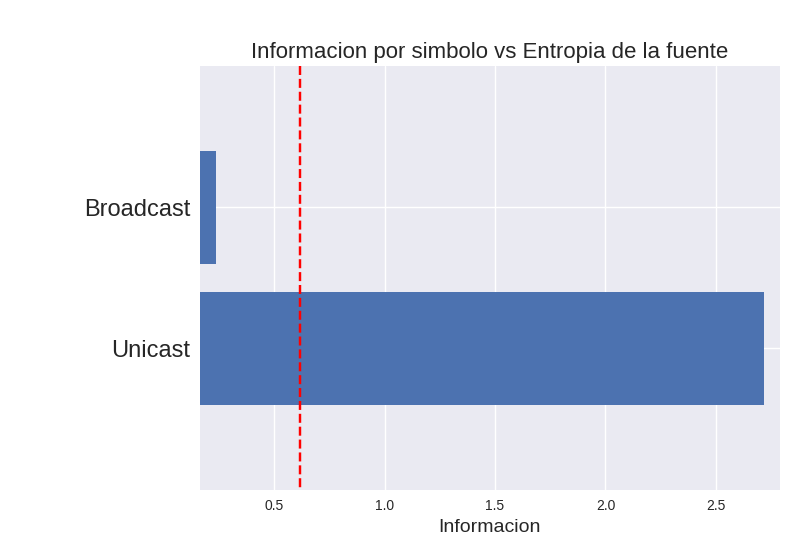
\includegraphics[width=\textwidth]{imagenes/mini_red/mini_red_unicastvsbroadcast.png}
  \end{subfigure}
  \label{fig:exp3_univsbr_infovsentro}
  \caption{Información de cada símbolo (Broadcast / Unicast) comparada con el valor de la entropía de la fuente de información (red local).}
\end{figure}

\par Con respecto al gráfico de barra de los hosts (figura 9), el equipo en el que se estuvo realizando la descarga tuvo una información muy baja y fue el único que estuvo por debajo de la entropía. Este resultado muestra una diferencia con las demás redes ya que el default gateway no resultó ser el de mayor probabilidad. Pero, es importante comentar que el host en el que se estaba iniciando una descarga envió paquetes ARP consultando por todas las direcciones posibles de la red. Por simplicidad del grafo no los incluimos a todas las direcciones de la red. También, en el grafo se puede ver una fuerte relación entre el host de la herramienta de monitoreo con el router como así también la de éste último con el equipo donde se estaba realizando la descarga.

\begin{figure}[h]
  \begin{subfigure}{.5\textwidth}
    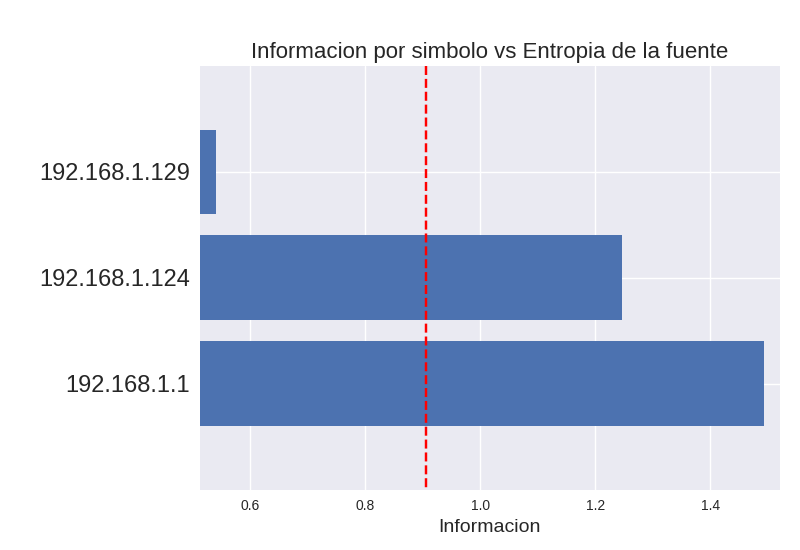
\includegraphics[width=\textwidth]{imagenes/mini_red/mini_red_hosts.png}
  \end{subfigure}
  \label{fig:exp3_hosts_infovsentro}
  \caption{Información de cada símbolo (host) comparada con el valor de la entropía de la fuente de información (red local).}
\end{figure}

\subsection{Conclusiones}

\par La entropía máxima es 0.5 ya que son 2 símbolos pero en este caso no se logró llegar a dicho valor. Esto sugiere que hay muchos envíos de mensajes de control, secuencia, etc. ya que éstos suelen ser broadcast. Este resultado está muy relacionado con el overhead de la red ya que los mensajes de control ocupan ancho de banda que, en algún caso, podrían enviarse datos.

\begin{figure}[h]
  \begin{subfigure}{.5\textwidth}
    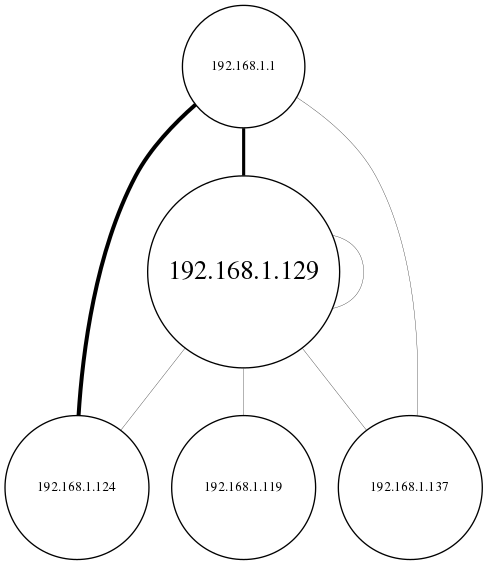
\includegraphics[width=\textwidth]{imagenes/mini_red/mini_red_Red.png}
  \end{subfigure}
  \label{fig:exp3_red}
  \caption{Diagrama de cómo creemos que está organizada la red de la tercer captura.}
\end{figure}

\par En esta red se puede distinguir solamente un nodo (\textbf{192.168.1.129}) pero fue un comportamiento por demás anómalo, por lo que no le podemos asignar ninguna función en especial dentro de la red. Creemos que si la captura hubiera durado alrededor de dos horas, el router (\textbf{192.168.124.1}) hubiera tenido mucha más participación. En particular por ser una red muy pequeña es esperable que se distinga un nodo, aunque si es inesperado qué nodo resultó ser.

\par Lamentablemente no hay una correspondencia entre lo que se conoce de la red y el resultado del experimento ya que la captura no duró lo suficiente y este outlier no nos permitió dilucidar la identidad de la puerta de enlace predeterminada.


\section{Cuarta captura: red intermedia}

\par En este último experimento, ejecutamos nuestro sniffer en una casa de comidas rápidas muy concurrida. La red es más grande que una hogareña pero más pequeña que la presentada en el primer experimento. La captura duró aproximadamente media hora.

\subsection{Resultados y análisis}

\par Como esta red posee muchísimos nodos decidimos realizar el gráfico con los que tienen menor información, en el mismo (figura 11) se pueden ver que hay algunos hosts con menos información que la entropía, mientras que hay otros que no. Pero en realidad todo los hosts restantes, es decir los que no fueron incluidos en el gráfico, tienen una información mayor. El host de la ip terminada en 110 es la puerta de enlace predeterminada, por lo cual es lógico que tenga mucha interacción con otros hosts. En la red hubo en total 127 hosts.

\begin{figure}[h]
  \begin{subfigure}{.5\textwidth}
    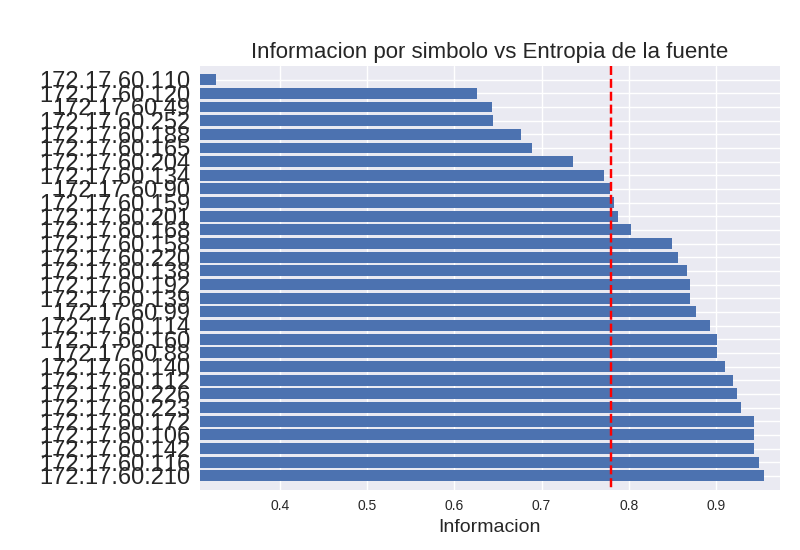
\includegraphics[width=\textwidth]{imagenes/mc/mchosts.png}
  \end{subfigure}
  \label{fig:exp4_hosts_infovsentro}
  \caption{Información de cada símbolo (host) comparada con el valor de la entropía de la fuente de información (red local).}
\end{figure}

\begin{figure*}[ht]
  \hspace*{-0.5cm}
  \begin{subfigure}{1.1\textwidth}
    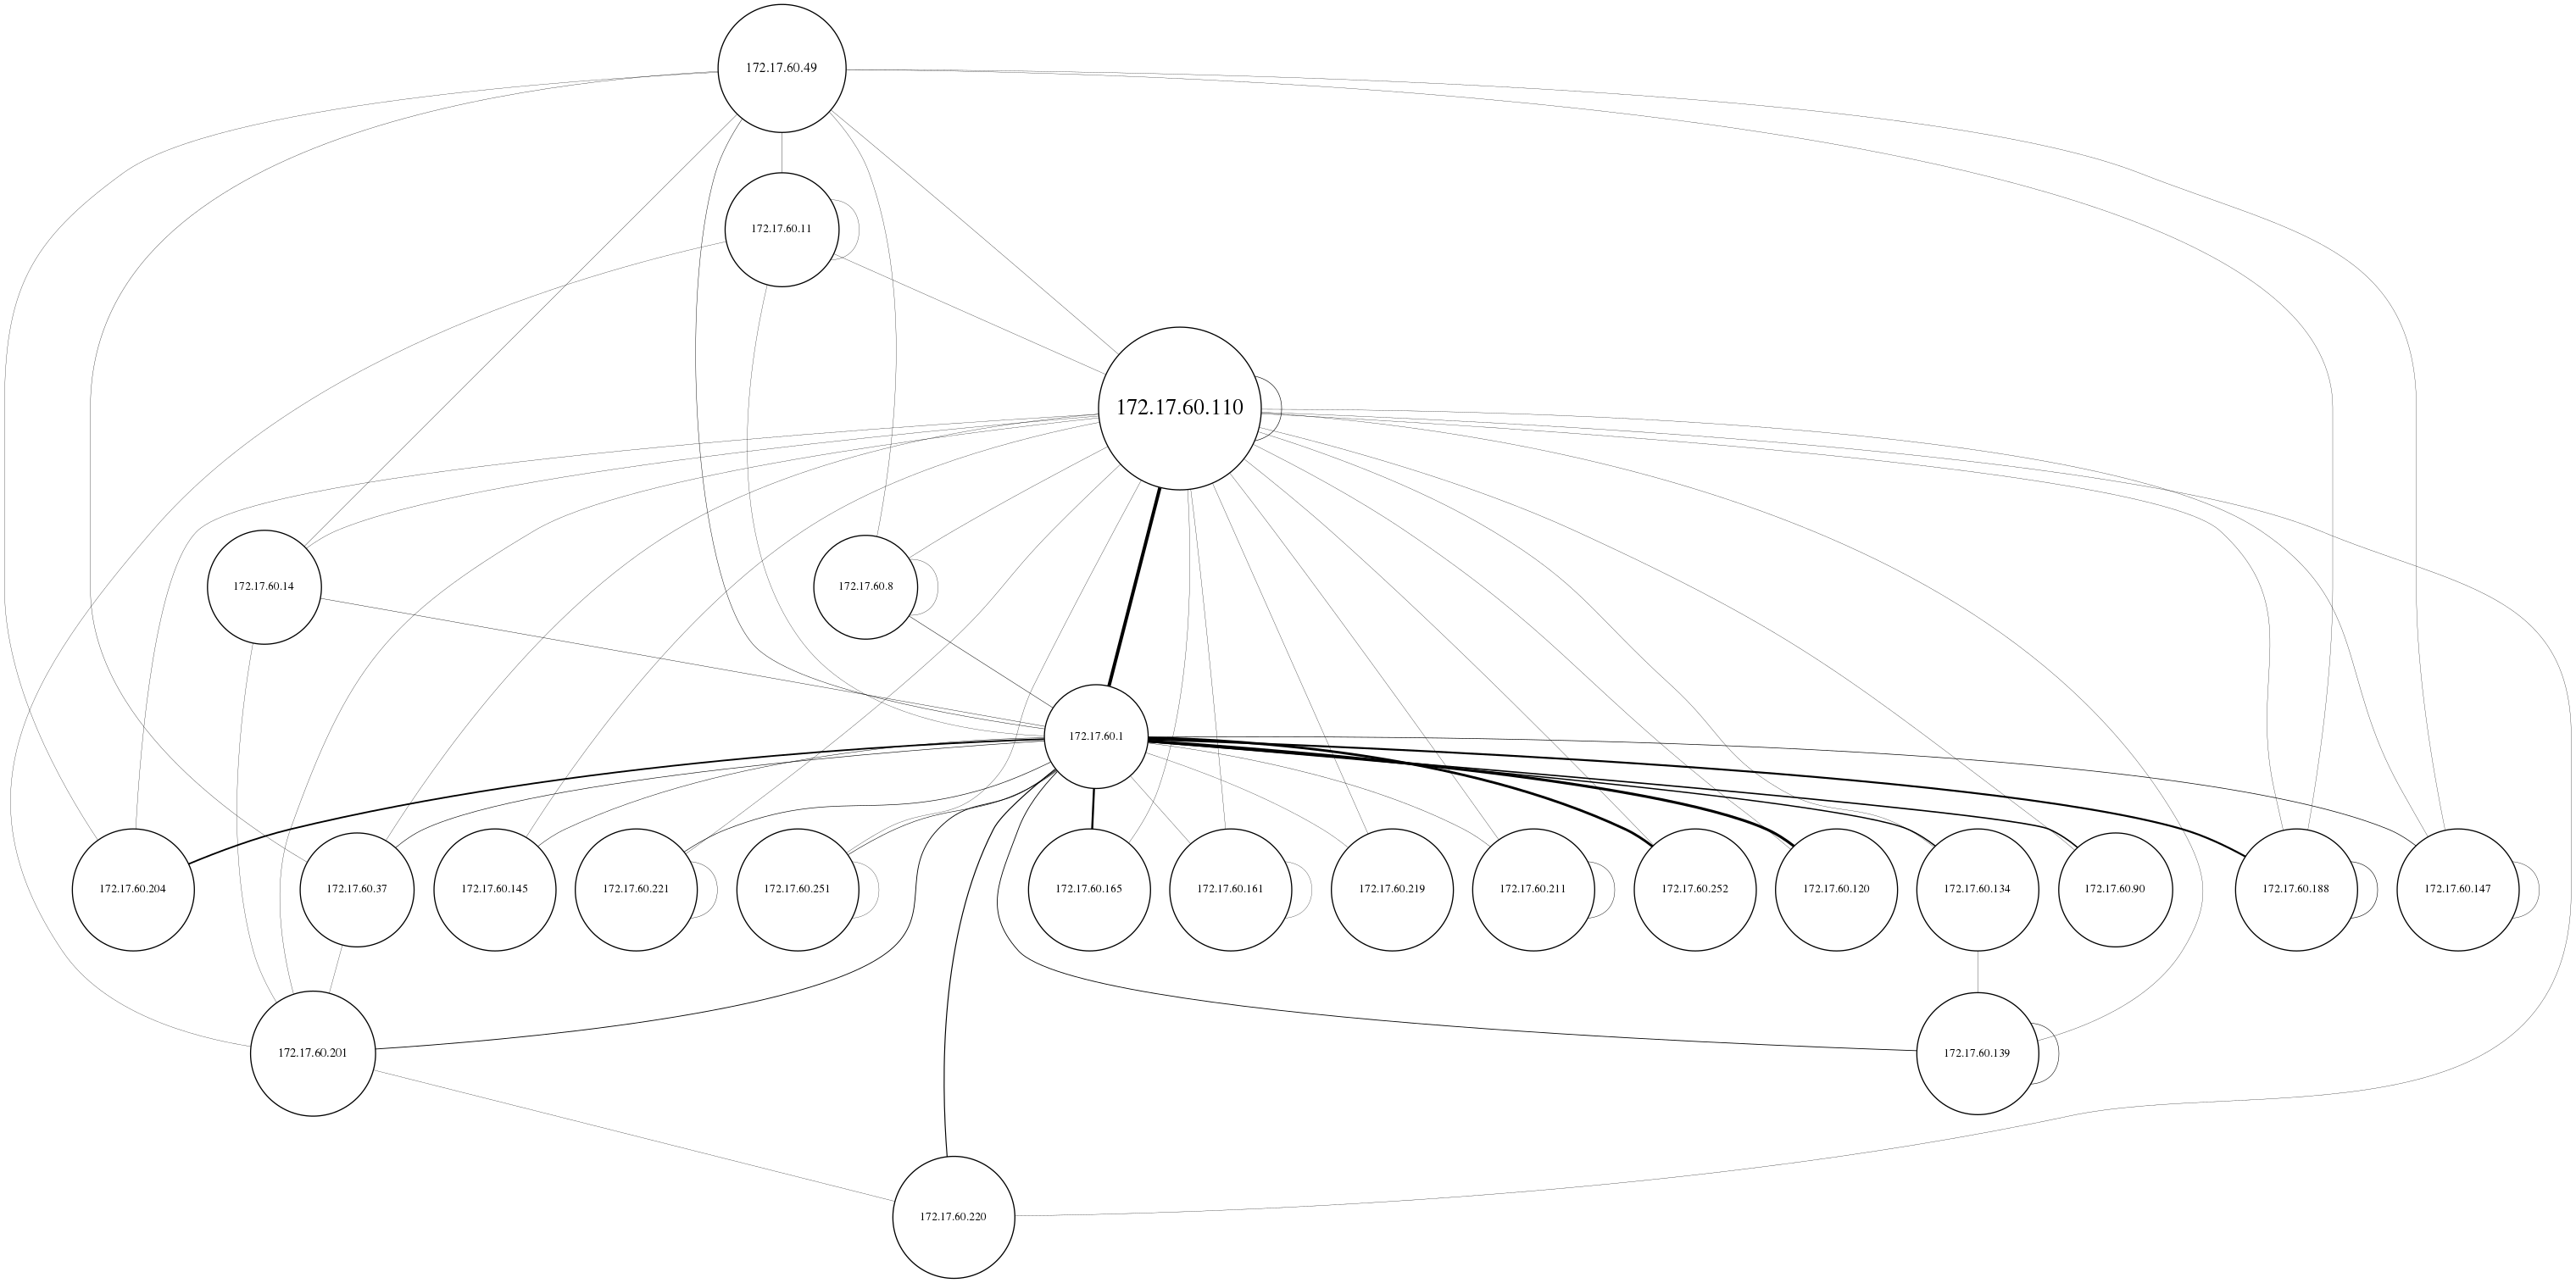
\includegraphics[width=\textwidth]{imagenes/mc/mcRed.png}
  \end{subfigure}
	\label{fig:exp4_grafo}
	\caption{Diagrama de cómo creemos que está organizada la red de la cuarta captura.}
\end{figure*}

\par Por otra parte, en el gráfico de barras en el que se compara la información de los paquetes \textit{Broadcast} contra la de los paquetes \textit{Unicast} (figura 12) se puede ver que hubo una gran diferencia a favor de la cantidad de paquetes broadcast en cuanto a paquetes enviados. Esto es sumamente razonable ya que la gran mayoría de los dispositivos conectados a la red son clientes.

\begin{figure}[h]
  \begin{subfigure}{.5\textwidth}
    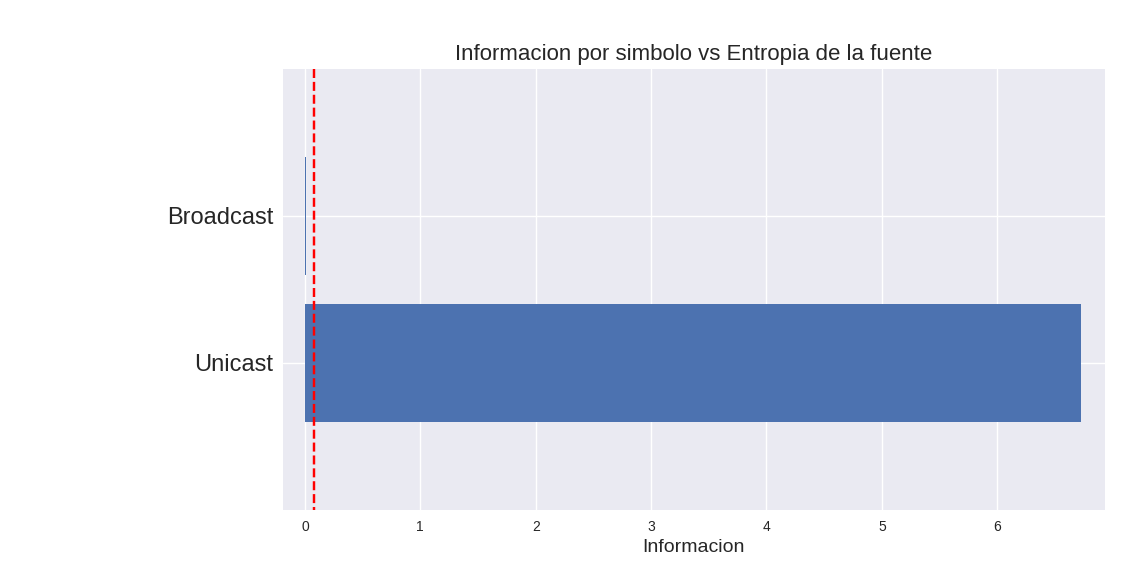
\includegraphics[width=\textwidth]{imagenes/mc/mcbrvsuni.png}
  \end{subfigure}
  \label{fig:exp4_univsbr_infovsentro}
  \caption{Información de cada símbolo (Broadcast / Unicast) comparada con el valor de la entropía de la fuente de información (red local).}
\end{figure}

\par Con respecto al grafo en el que mostramos los nodos distinguidos, podemos ver que el nodo \textbf{172.17.60.110} tiene muchísima más participación que el resto de los nodos. En particular, notamos que preguntó aproximadamente una vez por cada nodo pero, en cambio, sólo recibió preguntas de él mismo y del host \textbf{172.17.60.49}. Además, el nodo correspondiente al equipo cuya IP es \textbf{172.17.60.1} suele ser muy solicitado por la gran mayoría de los equipos de la red, pero en contrapartida éste no consultó en ningún momento por los demás.

\subsection{Conclusiones}
\par En este caso, la fuente S no tiene entropía máxima ya que hay muchos mensajes de control (por la gran cantidad de nodos activos que tiene la red). Además, por la longitud de la captura se acentuó esta tendencia, ya que muchos equipos no permanecieron durante toda la captura (recordemos que es un local de comida rápida). De esta manera hay mucho overhead en esta red.
\par En esta red se pudieron distinguir varios nodos (nueve en total). Son bastantes pocos con respecto al tamaño de la red pero, aún así, es razonable porque una red que tenga todos los nodos con un tráfico parejo no es conveniente. Pudimos notar que hubo un nodo que se comportó de manera no esperada, el nodo \textbf{172.17.60.1}. Este nodo hacía de intermediario entre la gran mayoría de los nodos de la red y el default gateway (\textbf{172.17.60.110}).
\par Gracias al resultado de la captura podemos afirmar que el default gateway es el equipo cuya ip es \textbf{172.17.60.110}. Nos convencemos también de que la herramienta también sirve para detectar puntos intermedios de paso hasta llegar al router.


\section{Conclusiones}
\section{Conclusiones generales}

\par En este informe realizamos un recorrido por cuatro tipos de redes locales con características y dimensiones distintas. La idea inicial era que las redes fueran bastante disímiles para poder contrastarlas e identificar rasgos que nos resulten llamativos. Nos basamos principalmente en el tamaño de la red y no en la tecnología de los equipos que se encontraban en ellas. Sin embargo, al trabajar sobre redes grandes notamos algunos factores que nos daban información sobre la organización de dichas redes y, luego de analizar esto, dimos una opinión sobre los posibles equipos que participan en ella.

\par Luego de observar el comportamiento de las redes con mayor cantidad de nodos, notamos que los mensajes Broadcast superan ampliamente a los mensajes Unicast. Esto se lo debemos, como es de esperarse, a los mensajes de control que se necesitan para mantener la red funcionando correctamente y pudimos notar el impacto directo que tiene en la información de dicho símbolo (\textit{Broadcast}). En contrapartida, la información de los mensajes Unicast es elevada, y todo esto hace que la entropía diste mucho mas de su valor máximo (\textit{0.5}).

\par Para el caso de la fuente S1, notamos que cuanto mas grande es la red, mas notamos la distinción de un nodo router o access point (que en general es planteado como el gran candidato a ser un nodo distinguido). De la misma manera, se observaron algunos otros nodos que se acercaban (que luego intentamos identificar como "organizadores" de la red) y muchos nodos que se comportan de manera similar (los host consumidores de la red).

\par Sobre la misma idea de distinguir nodos, este trabajo nos deja la idea de que la comparación de la información de los distintos símbolos (hosts) con la entropía de la fuente S1 puede brindarnos información relevante sobre los nodos distinguidos de la red. Y al seguir por ese camino, cuando ordenamos los hosts por su información notamos que varios, a pesar de posicionarse por encima de la entropía, también brindaban información sobre la organización de la red.




\end{document}
